\section*{Midterm 1 Review}

\subsection*{Transistors}

\begin{center} 
\begin{tabular}[t]{|c|c|p{200px}|}
\hline
Type & Drawing & Behavior \\ \hline
PMOS & \begin{circuitikz}[american] 
\draw (0, 0) node[pmos] (nmos) {};
\draw (nmos.G) node[left]{$G$};
\draw (nmos.S) node[left]{$S$};
\draw (nmos.D) node[left]{$D$};
\end{circuitikz} & Closed switch: gate voltage is at least $|V_{tp}|$ below source voltage (gate voltage is low).

Open switch: otherwise. \\ \hline

NMOS & \begin{circuitikz}[american] 
\draw (0, 0) node[nmos] (nmos) {};
\draw (nmos.G) node[left]{$G$};
\draw (nmos.S) node[left]{$S$};
\draw (nmos.D) node[left]{$D$};
\end{circuitikz} & 

Closed switch: gate voltage is at least $|V_{tn}|$ above source voltage (gate voltage is high).
\\ \hline
\end{tabular} \end{center}

\begin{center} \begin{tabular}{|c|c|c|c|}
\hline
Type & (Voltage-Controlled) Switch & Resistor-Switch & Resistor-Capacitor-Switch \\ \hline
PMOS & \begin{circuitikz}[scale=0.9]
			\draw (0, -2) node[label=left:$D$] {}
			to[switch, l_= $V_{GS} \leq -|V_{tp}|$, *-] (0,2)
			to[short, -*] ++(0, 0.2)
            node[label=right:$S$] {};;
			\draw (0, 2) -- (-1, 2)
			to[short, -*] ++(0, -2) node[label=left:$G$] {};;
			\draw (0, -1.75) to [short, -*, l=$V_{out}$] ++(1,0);;
		\end{circuitikz} & 
        \begin{circuitikz}[scale=0.9]
			\draw (0, -2) node[label=left:$D$] {}
			to[switch,l_= $V_{GS} \leq -|V_{tp}|$, *-] (0,0)
			to[R, l_=$R_{on}$, i<=$I_D$] ++(0, 2)
			to[short, -*] ++(0, 0.2) node[label=right:$S$] {};;
			\draw (0, 2) -- (-1, 2)
			to[short, -*] ++(0, -2) node[label=left:$G$] {};;
			\draw (0, -1.75) to [short, -*, l=$V_{out}$] ++(1,0);;
		\end{circuitikz} &
        \begin{circuitikz}[scale=0.9]
			\draw (0, -2) node[label=left:$D$] {}
			to[switch,l_= $V_{GS} \leq -|V_{tp}|$, *-] (0,0)
			to[R, l_=$R_{on}$, i<=$I_D$] ++(0, 2)
			to[short, -*] ++(0, 0.2)
            node[label=right:$S$] {};;
			\draw (0, 2) -- (-1, 2)
			to[C, -*, l_=$C_{GS}$] ++(0, -2) node[label=left:$G$] {};;
			\draw (0, -1.75) to [short, -*, l=$V_{out}$] ++(1,0);;
		\end{circuitikz} \\ \hline

NMOS &  \begin{circuitikz}[scale=0.9]
            \draw (0,-2)
            to[switch,l_= $V_{GS} \geq V_{tn}$]
            (0,2) to[short, -*] ++(0,0)
            node[label=left:$D$] {};;
            \draw (0,-2) -- (-1,-2)
            to[short, -*] ++(0,2) node[label=left:$G$] {};;
            \draw (0,1.75) to [short,-*,l=$V_{out}$] ++ (1,0);;
            \draw (0, -2) to [short, -*] ++(0, -0.2) node[label=right:$S$] {};;
        \end{circuitikz} &
        \begin{circuitikz}[scale=0.9]
            \draw (0,-2)
            to[switch,l_= $V_{GS} \geq V_{tn}$]
            (0,0) to[R,-*,l=$R_{on, N}$,i<=$I_D$] ++(0,2)
            node[label=left:$D$] {};;
            \draw (0,-2) -- (-1,-2)
            to[short, -*] ++(0,2) node[label=left:$G$] {};;
            \draw (0,1.75) to [short,-*,l=$V_{out}$] ++ (1,0);;
            \draw (0, -2) to [short, -*] ++(0, -0.2) node[label=right:$S$] {};;
        \end{circuitikz} & 
        \begin{circuitikz}[scale=0.9]
            \draw (0,-2)
            to[switch,l_= $V_{GS} \geq V_{tn}$]
            (0,0) to[R,-*,l=$R_{on, N}$,i<=$I_D$] ++(0,2)
            node[label=left:$D$] {};;
            \draw (0,-2) -- (-1,-2)
            to[C,-*,l=$C_{GS}$] ++(0,2) node[label=left:$G$] {};;
            \draw (0,1.75) to [short,-*,l=$V_{out}$] ++ (1,0);;
            \draw (0, -2) to [short, -*] ++(0, -0.2) node[label=right:$S$] {};;
        \end{circuitikz} \\ \hline
\end{tabular} \end{center}

\subsection*{First-Order Differential Equations}
\begin{enumerate}
    \item \textbf{Homogeneous Case}: the first derivative of the state variable $x(t)$ is proportional to the state variable by some constant $\lambda$. The general form of a homogeneous differential equation is:
    \begin{align*}
        \boxed{\frac{d}{dt} x(t) = \lambda x(t)}
    \end{align*}
    Given some initial state $x(0)$, the unique solution to this differential equation is:
    \begin{align*}
        \boxed{x(t) = x(0) e^{\lambda t}}
    \end{align*}

    \item \textbf{Non-homogenous Case}: the first derivative of the state variable $x(t)$ is equal to a scaled multiple of the state plus a nonzero constant. The general form of a non-homogeneous differential equation is:
    \begin{align*}
        \boxed{\frac{d}{dt} x(t) = \lambda x(t) + \alpha}
    \end{align*}
    To solve this type of differential equation, use a change of variables $x(t) = z(t) - \frac{\alpha}{\lambda}$. Plugging in this new definition of $x(t)$ into the original differential equation, we get the homogeneous case with respect to the new variable $z(t)$:
    \begin{align*}
        \frac{d}{dt} x(t) &= \lambda x(t) + \alpha \\
        \frac{d}{dt} (z(t) - \frac{\alpha}{\lambda}) &= \lambda (z(t) - \frac{\alpha}{\lambda}) + \alpha \\
        \frac{d}{dt} z(t) &= \lambda z(t)
    \end{align*}
    Now, you can use the result from the homogenous case to solve the differential equation in terms of $z(t)$, and then change variables back to $x(t)$ to get your final solution.
    \begin{align*}
        z(t) &= z(0) e^{\lambda t} \\
        x(t) + \frac{\alpha}{\lambda} &= (x(0) + \frac{\alpha}{\lambda}) e^{\lambda t} \\
    \end{align*}

    \vspace{-35px}
    $$\boxed{x(t) = x(0) e^{\lambda t} + \frac{\alpha}{\lambda}(e^{\lambda t} - 1)}$$

    \item \textbf{Non-homogeneous with Nonconstant Input $u(t)$}: the first derivative of the state variable is equal to a scalar multiple of the state plus a general non-constant function $u(t)$.
    \begin{align*}
        \boxed{\frac{d}{dt} x(t) = \lambda x(t) + u(t)}
    \end{align*}
    The solution to this differential equation is:
    \begin{align*}
        \boxed{x(t) = x(0) e^{\lambda t} + \int_0^t u(\tau) e^{\lambda(t - \tau)} \, d\tau}
    \end{align*}
\end{enumerate}
\newpage 
\subsection*{Time-Domain RC circuits}
\begin{figure}[H]
	\begin{center}
		\begin{circuitikz}
			\draw (0, 4)
			to[V =$V_s$] (0, 0);
			\draw (0, 4)
			to[switch,l^=\mbox{$t = 0$}](3,4)
			(3,4) to[R = $R$,v=$V_R(t)$,i>^=$i_R(t)$] (6,4)	
			to [short] (8,4)
			to[C = $C$, v=$V_{C}(t)$,i>^=$i_C(t)$] (8,0)
			to [short] (0,0);
		\end{circuitikz}
		\caption{\label{fig:circuit}RC Circuit with Voltage Source}
	\end{center}
\end{figure}

\begin{enumerate}
    \item \textbf{Step 1}: Use KCL and KVL equations, and the capacitor charge-voltage relationship ($i_C(t) = C \frac{d}{dt} V_C(t)$) to get a differential equation in terms of the given variable (typically $V_C(t)$ or $i_C(t)$).
    
    For the above circuit, KCL gives us the following differential equation:
    \begin{align*}
        i_R(t) &= i_C(t) \\
        \frac{V_s - V_C(t)}{R} &= C \frac{d}{dt} V_C(t)
    \end{align*}

    \item \textbf{Step 2}: Identify the differential equation as homogenous, non-homogenous, or having a non-constant input, and solve the differential equation using the tools above.

    We can express the above differential equation the form:
    \begin{align*}
        \frac{d}{dt} V_C(t) = -\frac{1}{RC} V_C(t) + \frac{1}{RC} V_s
    \end{align*}

    How would you solve this differential equation if $V_s = 0$? $V_s = V_{DD} > 0$? $V_s(t) = e^{t}$?

    \item \textbf{Step 3}: Plug initial conditions into your solution.

    For example, uncharged capacitors have an initial condition $V_C(t = 0) = 0$.
\end{enumerate}

Note: Circuits with inductors can be solved in a similar manner, using the inductor I-V relationship: 
$$\boxed{V_L(t) = L \frac{d}{dt} i_L(t)}$$

\newpage
\subsection*{Diagonalization and Eigenbasis}

Given a system of the form
\begin{align*}
    \vec{y} = A \vec{x}
\end{align*}
We define the eigenbasis as
\begin{align*}
    V = \begin{bmatrix}
        \vec{v_1} & \vec{v_2} & \dots & \vec{v_n}
    \end{bmatrix}
\end{align*}
where $\vec{v_i}$ is the $i^{\text{th}}$ eigenvector of $A$ \\
Then, we can express any vector as a linear combination of eigenvectors of $A$
\begin{align*}
    \vec{x} = a_1 \vec{v_1} + \dots + \vec{v_n} \\
    \vec{x} = V \vec{\widetilde{x}} \\
    \vec{\widetilde{x}} = V^{-1} \vec{x}
\end{align*}
Then, if we substitute $V \vec{\widetilde{x}}$ for $\vec{x}$ in our system, we get
\begin{align*}
    V \vec{\widetilde{y}} = AV \vec{\widetilde{x}} \\
    \vec{\widetilde{y}} = V^{-1}AV \vec{\widetilde{x}}
\end{align*}

Because $V$ is the eigenbasis, $V^{-1}AV$ is diagonal
\begin{align*}
    V^{-1}AV = 
    \begin{bmatrix}
        \lambda_1 & 0 & \dots & 0 \\
        0 & \lambda_2 & \dots & 0 \\
        \vdots & \vdots & \ddots & \vdots \\
        0 & 0 & \dots & \lambda_n
    \end{bmatrix}
\end{align*}

You may find this diagram useful to visualize this process:
\begin{figure}[H]
    \centering
    \begin{tikzpicture}[node distance = 2cm, thick, every node/.style={inner sep=0.25em,outer sep=0.25em}]%
      \node (1) [circle,draw,minimum size=2em] {$\vec{x}$};
      \node (2) [circle,draw,right=of 1,minimum size=2em] {$\vec{y}$};
      \node (3) [circle,draw,below=of 2,minimum size=2em] {$\widetilde{\vec{y}}$};
      \node (4) [circle,draw,below=of 1,minimum size=2em] {$\widetilde{\vec{x}}$};
      \draw[->] (1) -- node [rectangle,draw,midway,above,minimum size=2.5em] {$A$} (2);
      \draw[->] (1.240) -- node [rectangle,draw,midway,left,minimum size=2.5em]{$V^{-1}$} (4.120);
      \draw[->] (4.60) -- node [rectangle,draw,midway,right,minimum size=2.5em]{$V$} (1.300);
      \draw[->] (2.300) -- node [rectangle,draw,midway,right,minimum size=2.5em]{$V^{-1}$} (3.60);
      \draw[->] (3.120) -- node [rectangle,draw,midway,left,minimum size=2.5em]{$V$} (2.240);
      \draw[->] (4) -- node [rectangle,draw,midway,below,minimum size=2.5em] {$D$} (3);
    \end{tikzpicture}%
\end{figure}

\subsection*{Multivariate ODEs}
When given a system of differential equations of the form
\begin{align*}
    \frac{d}{dt} \vec{x}(t) = 
    A \vec{x}(t)
\end{align*}
you can diagonalize the system and solve in the eigenbasis.

\begin{enumerate}
    \item \textbf{Step 1}: Find the eigenvalue-eigenvector pairs $(\lambda_1, \vec{v_1}), \dots (\lambda_n, \vec{v_n})$ of your $A$ matrix.
    \item \textbf{Step 2}: Define $V = \begin{bmatrix}
        \vec{v_1} & \vec{v_2} & \dots & \vec{v_n}
    \end{bmatrix}$, and transform your system to the eigenbasis

    \begin{align*}
    \frac{d}{dt} \vec{\widetilde{x}}(t) =  V^{-1}AV \vec{\widetilde{x}}(t) =
    \begin{bmatrix}
        \lambda_1 & 0 & \dots & 0 \\
        0 & \lambda_2 & \dots & 0 \\
        \vdots & \vdots & \ddots & \vdots \\
        0 & 0 & \dots & \lambda_n
    \end{bmatrix} \vec{\widetilde{x}}(t) \\
    \vec{\widetilde{x}}(0) = V^{-1} \vec{x}(0)
    \end{align*}

    \item We can then decompose this matrix-vector equation into several single-variable equations
    \begin{align*}
        \frac{d}{dt} \widetilde{x_1}(t) = \lambda_1 \widetilde{x_1}(t) \\
        \dots \\
        \frac{d}{dt} \widetilde{x_n}(t) = \lambda_n \widetilde{x_n}(t)
    \end{align*}
    Solve each equation to get expressions for $\widetilde{x_1}, \dots \widetilde{x_n}$
    \begin{align*}
        \widetilde{x_1}(t) = \widetilde{x_1}(0) e^{\lambda_1 t} \\
        \dots \\
        \widetilde{x_n}(t) = \widetilde{x_1}(0) e^{\lambda_n t} 
    \end{align*}

    \item Transform your solution back to the standard basis
    \begin{align*}
        \vec{x}(t) = V \vec{\widetilde{x}}(t)
    \end{align*}

\end{enumerate}

\textbf{Second-Order ODE}: If we have a differential equation that depends on $\frac{d^2}{dt^2} x$, define your state vector as $\begin{bmatrix} x \\ \frac{d}{dt} x \end{bmatrix}$ and solve your system as a Multivariate ODE.

\textbf{Complex Eigenvalues}: The behavior of a system (for example, a RLC circult) in the time domain varies based on whether its eigenvalues are real, imaginary, or complex.
\begin{enumerate}
    \item \textit{Real}: The time-domain response is a decaying exponential with no oscillations.
    \item \textit{Imaginary}: The response is a sinusoid that oscillates without decaying.
    \item \textit{Complex}: The response is the product of a decaying exponential and a sinusoid, so it oscillates as it decays.
\end{enumerate}

\subsection*{Complex Numbers}
\textbf{Complex number representations:} You can either represent complex numbers in 
\begin{enumerate}
    \item rectangular form ($a + bi$, where $a$ is the real component and $b$ is the imaginary component), or
    \item polar form ($Me^{j \theta}$, where $M$ is the magnitude and $\theta$ is the angle)
\end{enumerate}

\textbf{Operations with complex numbers}
\begin{enumerate}
    \item To go from rectangular to polar
    \begin{align*}
        M = \sqrt{a^2 + b^2} \\
        \theta = \atan2(b, a)
    \end{align*}
    \textit{Note: atan2(y, x) returns the angle between y and x. It is like arctan, except its range is from 0 to $2\pi$}
    \item To go from polar to rectangular
    \begin{align*}
        a = M\cos(\theta) \\
        b = M\sin(\theta)
    \end{align*}

    \item It is easiest to add two numbers in rectangular form: the real and imaginary components add
    \begin{align*}
        (a + bj) + (c + dj) = (a + c) + (b + d)j
    \end{align*}

    \item It is easiest to multiple numbers in polar form: the magntudes multiply and the phases add
    \begin{align*}
        (M_1 e^{j \theta_1})(M_2 e^{j \theta_2}) = M_1 M_2 e^{j (\theta_1 + \theta_2)}
    \end{align*}
\end{enumerate}

\textbf{Euler's Identity}: Euler's Identity relates complex exponentials (the polar representation of complex numbers) to sines and cosines.
\begin{align*}
    e^{j \theta} = \cos(\theta) + j \sin(\theta)
\end{align*}

\subsection*{Frequency Domain Analysis: Phasors and Impedance}
We can analyze circuits with sinusoidal inputs/sources in the frequency domain. To do so, we use the \textit{phasor} representation of sinusoidal voltages and currents, and the \textit{impedances} of passive circuit elements (resistors, capacitors, inductors).

\begin{enumerate}
    \item \textbf{Find the phasor representations of voltages and currents}: 
    Let 
    \begin{align*}
    V_s = A\cos(\omega t + \phi)
    \end{align*}

    where A is the amplitude of the wave, $\omega$ is the angular frequency in radians per second, and $\phi$ is the phase offset. \\
    Then, the phasor representation of $V_s$ is as follows

    \begin{align*}
    \widetilde{V_s} = A e^{j \phi}
    \end{align*}
    \textit{Note:} to find the phasor representation of a sine wave, first convert to cosine: $\sin(\theta) = \cos(\theta - \pi/2)$ \\

    \item \textbf{Find the impedance of passive circuit elements}:
    The impedance of a circuit element is defined as its current-voltage relationship in the phasor domain.
    \begin{align*}
    Z = \frac{\widetilde{V}}{\widetilde{I}}
    \end{align*}
    
    \begin{center}
        \begin{tabular}[t]{|c|c|c|}
        \hline
        Element & Drawing & Impedance \\ \hline
        Resistor & 
        \begin{circuitikz}
            \draw (0, 0) to[R = $R$] (2,0);
        \end{circuitikz}
        & $Z_R = R$ \\ \hline
        Capacitor & \begin{circuitikz}
            \draw (0, 0) to[C = $C$] (2,0);
        \end{circuitikz}
        & $Z_C = \frac{1}{j \omega C}$ \\ \hline
        Inductor & \begin{circuitikz}
            \draw (0, 0) to[L = $L$] (2,0);
        \end{circuitikz}
        & $Z_L = j \omega L$ \\ \hline
        \end{tabular}
    \end{center}

    \item \textbf{Solve}: Use KCL, KVL, and impedance relationships to solve for the output voltage.
    If necessary, convert the output voltage back to the time domain ($Ae^{j \phi}$ at frequency $\omega$ becomes $A\cos(\omega t + \phi)$)
\end{enumerate}

\subsection*{Transfer Functions and Filters}
When we want to look at the input-output relationship of a circuit, we look at its transfer function, which is usually defined as
\begin{align*}
    H(\omega) = \frac{\widetilde{V}_{out}}{\widetilde{V}_{in}}
\end{align*}

A \textbf{filter} is a circuit that only lets some frequencies pass through and attenuates the rest.

\begin{center}
    \begin{tabular}[t]{|c|c|c|c|c|}
        \hline
        Type & \multicolumn{2}{c|}{Circuit} & \multicolumn{2}{c|}{Transfer Function}\\ \hline
        Low-Pass & 
        \begin{circuitikz}
            \draw (0, 2) node[label=left:$\widetilde{V}_{in}$] {}
            to[R = $R$] (2,2) node[label=right:$\widetilde{V}_{out}$] {};
            \draw (2, 2) to[C = $\frac{1}{j \omega C}$] (2, 0.5)
            node[ground] {};
        \end{circuitikz} &
        \begin{circuitikz}
            \draw (0, 2) node[label=left:$\widetilde{V}_{in}$] {}
            to[L = $j \omega L$] (2,2) node[label=right:$\widetilde{V}_{out}$] {};
            \draw (2, 2) to[R = $R$] (2, 0.5)
            node[ground] {};
        \end{circuitikz} & 
        $H(\omega) = \frac{1}{1 + j \omega RC}$ &
        $H(\omega) = \frac{1}{1 + j \omega L/R}$ \\ \hline

        High-Pass & 
        \begin{circuitikz}
            \draw (0, 2) node[label=left:$\widetilde{V}_{in}$] {}
            to[C = $\frac{1}{j \omega C}$] (2,2) node[label=right:$\widetilde{V}_{out}$] {};
            \draw (2, 2) to[R = $R$] (2, 0.5)
            node[ground] {};
        \end{circuitikz} &
        \begin{circuitikz}
            \draw (0, 2) node[label=left:$\widetilde{V}_{in}$] {}
            to[R = $R$] (2,2) node[label=right:$\widetilde{V}_{out}$] {};
            \draw (2, 2) to[L = $j \omega L$] (2, 0.5)
            node[ground] {};
        \end{circuitikz} & 
        $H(\omega) = \frac{j \omega RC}{1 + j \omega RC}$ &
        $H(\omega) = \frac{j \omega L/R}{1 + j \omega L/R}$ \\ \hline

        Band-Pass & \multicolumn{2}{c|}{
            \begin{circuitikz}
                \draw (0, 2.5) node[label=left:$\widetilde{V}_{in}$] {}
                to[R = $R$] (2,2.5);
                \draw (2, 2.5) to[C = $\frac{1}{j \omega C}$] (2, 0)
                node[ground] {};
                \draw (2, 2.5) to[short] (3.5, 2.5)
                node[op amp, yscale=-1, anchor=+](A1) {};
                \draw (A1.-) to[short] (3.5, 0.75)
                to[short] (5.75, 0.75)
                to[short] (5.75, 2);
                \draw (A1.out) to[C = $\frac{1}{j \omega C}$] (7.5, 2)
                node[label=right:$\widetilde{V}_{out}$] {};
                \draw (7.5, 2) to[R = $R$] (7.5, 0)
                node[ground] {};
            \end{circuitikz}
            } &
            \multicolumn{2}{c|}{
                $H(\omega) = \frac{j \omega RC}{1 + j \omega RC} \cdot \frac{1}{1 + j \omega RC}$
            } \\ \hline
    \end{tabular}
\end{center}
\textit{Note}: For a general band-pass filter, you connect a high-pass and a low-pass filter with a unity gain buffer in between. The transfer function of the band-pass filter is the product of the transfer functions of the two filters it is made of.

\subsection*{Resonance}
Consider an LRC circuit in the frequency domain
\begin{center}
    \begin{circuitikz}
        \draw (0, 2) node[label=left:$\widetilde{V}_{in}$] {}
        to[L = $j \omega L$] (2,2);
        \draw (2, 2) to[R = $R$] (4.5, 2)
        node[label=right:$\widetilde{V}_{out}$] {};
        \draw (4.5, 2) to[C = $\frac{1}{j \omega C}$] (4.5, 0.5)
        node[ground] {};
    \end{circuitikz}
\end{center}

If out output is the voltage over the capacitor, the transfer function of this circuit is as follows
\begin{align*}
    H(\omega) = \frac{1/LC}{(j \omega)^2 + j \omega R/L + 1/LC}
\end{align*}

We degine $\omega_n = \sqrt{1/LC}$ to be the \textit{resonant frequency} of the circuit.
At this frequency, the impedances of the capacitor and inductor "cancel out" ($j \omega L = \frac{1}{j \omega C}$), resulting in a spike in the magnitude of the transfer function.

\begin{align*}
    H(\omega_n = \sqrt{1/LC}) = \frac{1/LC}{j\sqrt{\frac{1}{LC}} \frac{R}{L}}
\end{align*}

For an LRC bandpass filter with $\omega_n = 10^4$, the magnitude of the transfer function would look something like this (\textit{Note: the plot is on a log-log scale}) \\
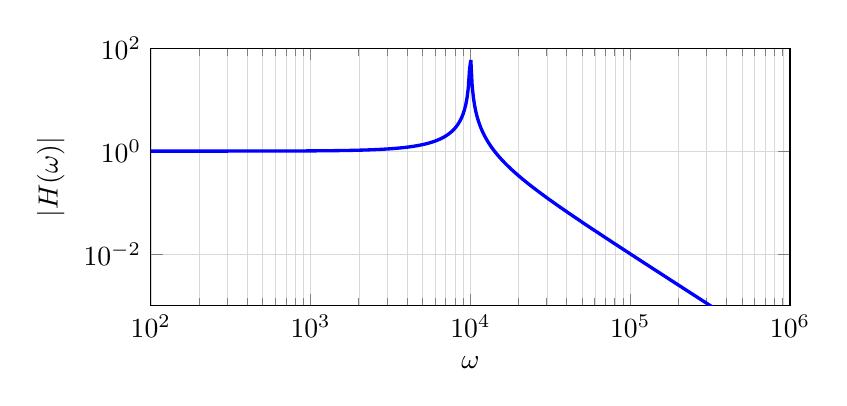
\begin{tikzpicture}[
    declare function={
    mag(\omega)= (10^8) / (sqrt((10^8 - \omega^2)^2 + (\omega * 100)^2))
    ;
    }
]
    \begin{loglogaxis}
    [
    ymin=0.001, ymax=100, ylabel=$|H(\omega)|$,
    xmin=10^2, xmax=10^6, xlabel=$\omega$,
    domain=10^2:10^6,
    grid=both, grid style={line width=.1pt, draw=gray!30},
    width=\textwidth * 0.8,
    height=\textwidth / 2.5,
    samples=500
    ]
    \addplot [blue,very thick] {mag(x)};
    \end{loglogaxis}
\end{tikzpicture}
